\documentclass[12pt]{article}
\usepackage[a4paper,margin=1in]{geometry}
\usepackage{amsmath,amssymb}
\usepackage{graphicx}
\usepackage{siunitx}
\sisetup{per-mode=symbol}


\title{Matrix 1.7.1}
\author{ai25btech11015 -- M Sai Rithik}
\date{}

\begin{document}
\maketitle

\section*{Question}
Show that the points \((0,0)\), \((2m,-4)\), and \((3,6)\) are collinear, and hence find \(m\), using the rank method.

\section*{Solution}

Let the given points be
\[
A = (0,0), \quad B = (2m,-4), \quad C = (3,6).
\]

\subsection*{Step 1: Form vectors}
\[
AB = B - A = \begin{bmatrix} 2m \\ -4 \end{bmatrix}, 
\quad AC = C - A = \begin{bmatrix} 3 \\ 6 \end{bmatrix}.
\]

\subsection*{Step 2: Matrix form}
Construct the matrix
\[
M = \begin{bmatrix}
2m & 3 \\
-4 & 6
\end{bmatrix}.
\]

For the points to be collinear, the two vectors \(AB\) and \(AC\) must be linearly dependent.  
This means
\[
\text{rank}(M) = 1 \quad \Leftrightarrow \quad \det(M) = 0.
\]

\subsection*{Step 3: Determinant condition}
\[
\det(M) = (2m)(6) - (-4)(3) = 12m + 12.
\]

Setting this equal to zero:
\[
12m + 12 = 0 \quad \Rightarrow \quad m = -1.
\]

\section*{Final Answer}
The given points are collinear when
\[
\boxed{m = -1}
\]

\begin{center}
\end{center}

\begin{figure}[h!]
    \centering
    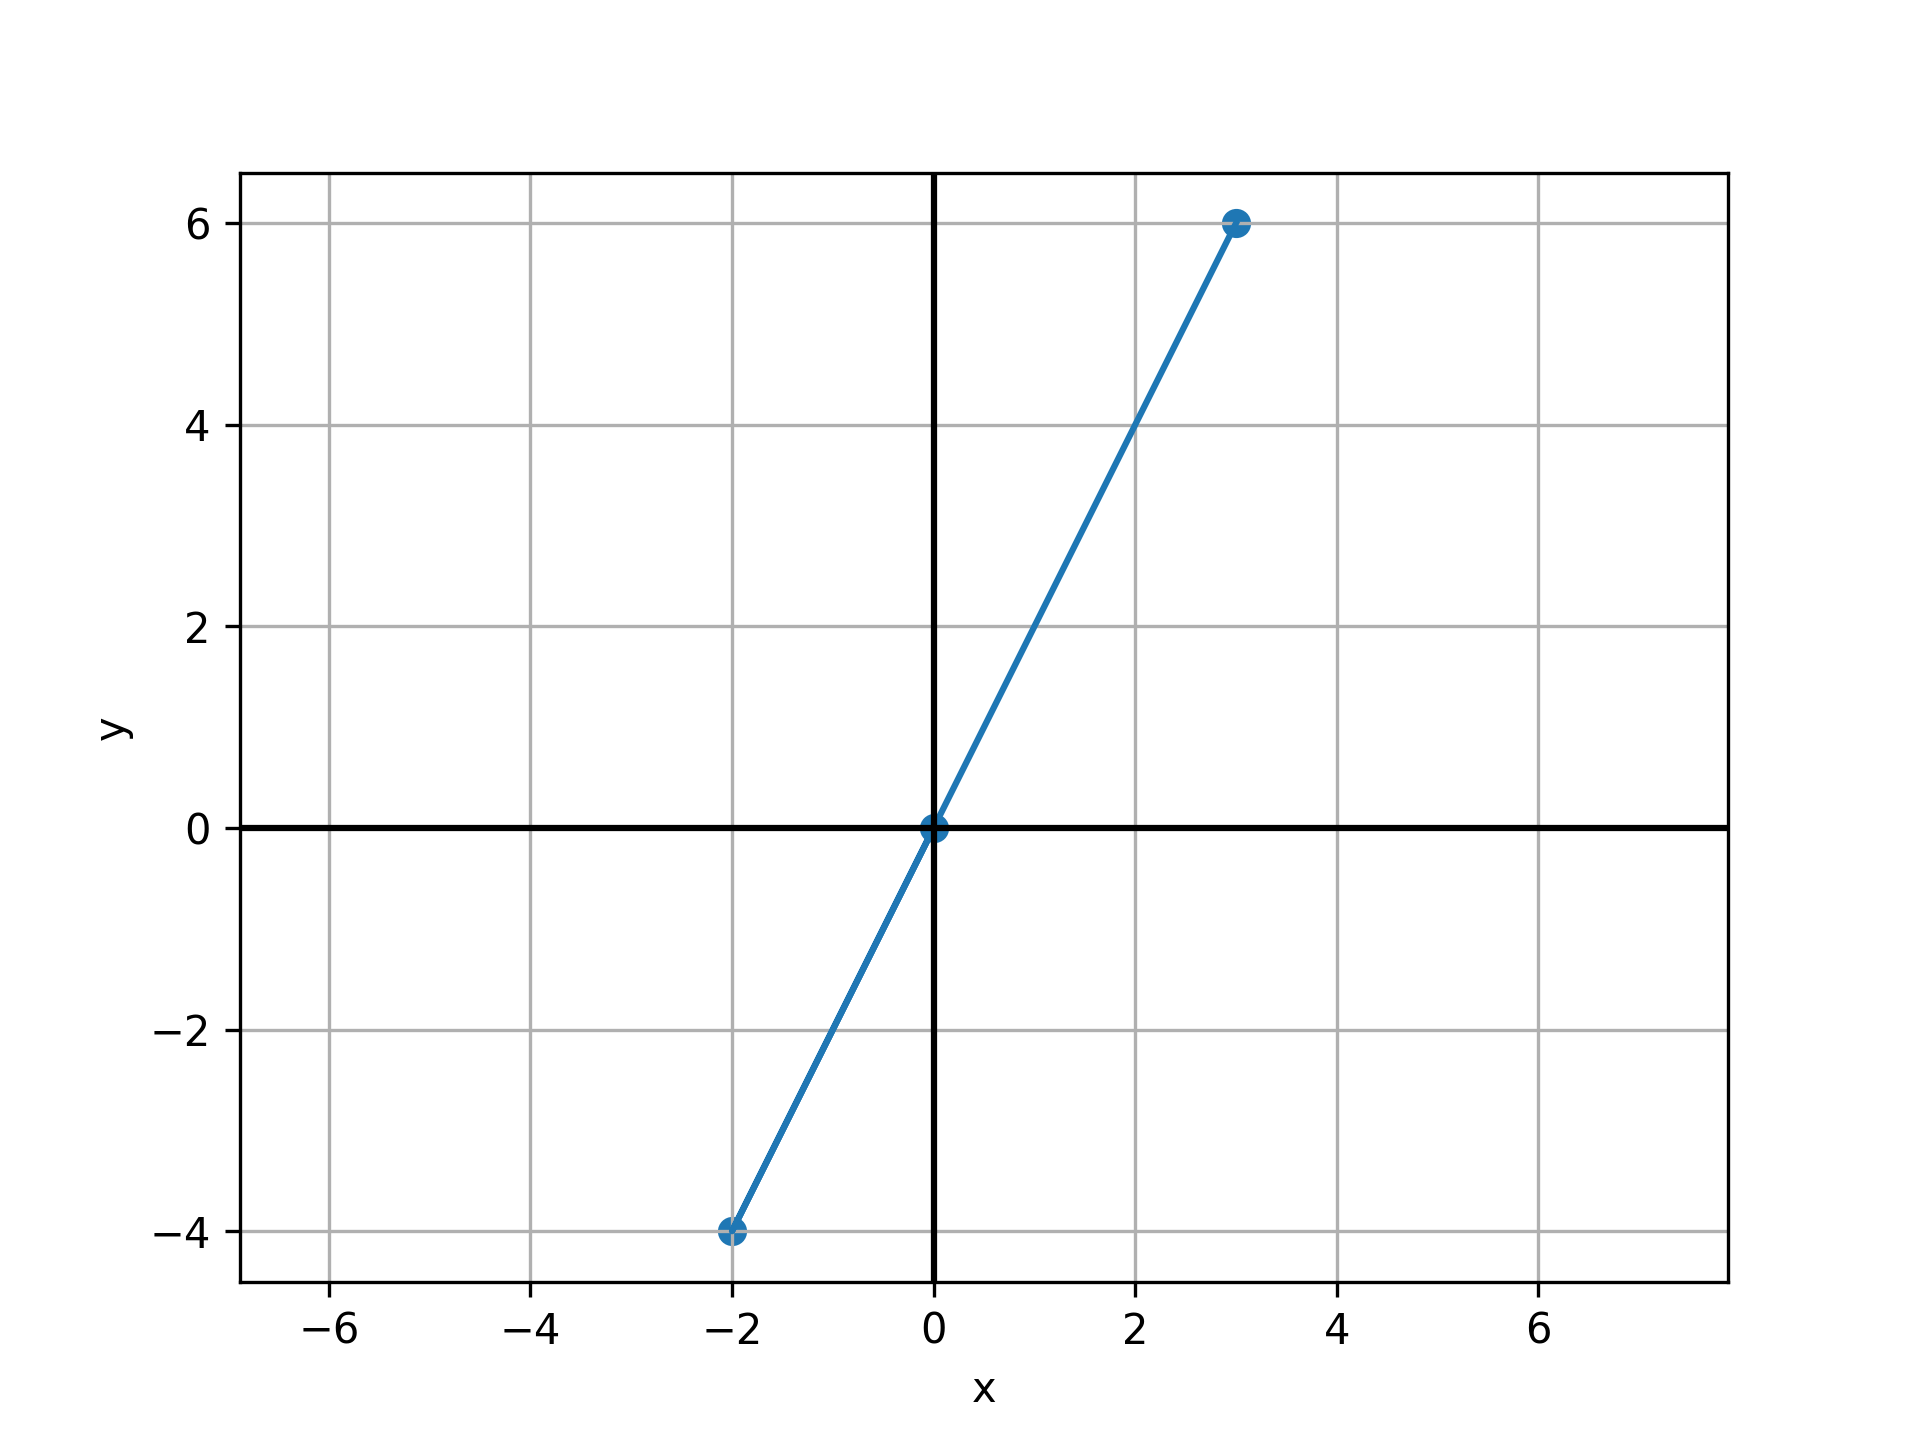
\includegraphics[width=0.65\linewidth]{figs/fig.png}
    \caption{Graph}
\end{figure}

\end{document}
